% =============================================================================
\chapter{Quantum noise in BEC interferometry}
\label{cha:bec-noise}
% =============================================================================

BECs are macroscopic quantum objects and can be potentially used as high precision interferometric detectors and sensors.
Unlike photons, atoms can interact strongly, leading to loss of coherence and decreased interferometric contrast.
An accurate quantitative model for these quantum many-body effects is essential for explaining the results of atom interferometry experiments and for planning the future ones.

In this chapter we will apply the truncated Wigner method from \charef{wigner-bec} to the task of simulating the dynamics of such experiments.
We will start from describing the mean-field approach leading to the conventional Gross-Pitaevskii equations (\abbrev{gpe}s)~\cite{Pitaevskii2003}.
We then extend it to include quantum effects, such as the noise from linear and nonlinear losses.
The accurate description of nonlinear losses is especially important as their relative effect increases when atom numbers are increased to improve contrast.

We will compare the effect of quantum fluctuations and technical noises, such as imperfect measurements or coupling phase and amplitude uncertainty, on the interferometric contrast.
We will also consider the experimental measurement process of the contrast in detail and investigate the influence of quantum effects on such an important characteristic as the phase noise.

% =============================================================================
\section{Two-component trapped BEC}
\label{sec:bec-noise:system}
% =============================================================================

The system we are interested in is an ultracold harmonically trapped \Rb{} \abbrev{bec} in $3$ effective dimensions such as the one used in the experiments by Riedel \textit{et~al}~\cite{Riedel2010} and Egorov \textit{et~al}~\cite{Egorov2011,Egorov2013}.
The \abbrev{bec} in question has two components with a significant nonlinear repulsive interaction (both inter- and intra-component), nonlinear losses and perhaps some additional linear unitary effects, such as an electromagnetic coupling between components.
The number of components is only set to two in order to simplify the resulting equations for the experiments described in this chapter; it can be easily increased if necessary.

We assume that the \abbrev{bec} has $s$-wave interactions, which makes the nonlinear interaction coefficients have the form
\begin{eqn}
\label{eqn:bec-noise:system:g}
    g_{jk} = \frac{4\pi\hbar^2 a_{jk}}{m},
\end{eqn}
where $j$ and $k$ are the indices of the interacting components, $a_{jk}$ is the corresponding $s$-wave scattering length, and $m$ hereinafter in this chapter stands for the mass of a \Rb{} atom.
Here we assume a momentum cutoff $k_d \ll 1 / a_{jk}$ in the numerical simulations, otherwise the couplings must be renormalized~\cite{Sinatra2002}.

The external harmonic trapping potential $V_j$ for the component $j$ (which can include a component-dependent shift along some of the axes) has the form
\begin{eqn}
\label{eqn:bec-noise:system:V}
    V_j
    = \frac{m}{2} \sum_{d=1}^3 \omega_d^2 (x_d - l_d)^2,
\end{eqn}
where $\omega_d$ are trapping frequencies, which will be specified later when the concrete experiments are described.

Again, in principle, the methods described in this chapter can be easily generalized to include an arbitrary potential shape, and possibly some different form of nonlinear interaction coefficients, but for the experiments to be described the equations above will apply.

% =============================================================================
\section{Mean-field approximation}
% =============================================================================

We will start from the classical model of the trapped \abbrev{bec} --- the mean-field approximation.
While it cannot predict quantum effects, it provides the basis for comparison with the truncated Wigner method, and can be also applied to calculate the ground state of a trapped \abbrev{bec} numerically.


% =============================================================================
\subsection{Two-component condensate}
% =============================================================================

Hereafter we are discussing $^{87}$Rb condensate and two of its $5^2S_{1/2}$ states: $\vert1,-1\rangle$ and $\vert2,1\rangle$,
called $\vert1\rangle$ and $\vert2\rangle$, correspondingly.
The energy of the mixture of two states is~\cite{Pitaevskii2003}:
\begin{eqn}
\label{eqn:mean-field:two-comp-energy}
	E(\Psi) = & \int\limits_V \left(
		- \frac{\hbar^2 \Psi_1^* \nabla^2 \Psi_1}{2m}
		- \frac{\hbar^2 \Psi_2^* \nabla^2 \Psi_2}{22m}
	\right. \\
	& \left.
		+ (V_1 + \hbar \omega_1) n_1 + (V_2 + \hbar \omega_2) n_2
		+ \frac{g_{11}}{2} n_1^2 + \frac{g_{22}}{2} n_2^2 + g_{12} n_1 n_2
	\right) d\xvec.
\end{eqn}
External trap potential $V_1$ and $V_2$ can be different for each component, depending on experimental setup.
Interaction coefficients $g_{11}$, $g_{12}$ and $g_{22}$ depend on corresponding scattering lengths:
\[
	g_{ij} = \frac{4 \pi \hbar^2 a_{ij}}{m}.
\]
The quantity $\omega_{hf}$ is the hyperfine splitting for $5^2S_{1/2}$ and equals
$\omega_{hf} \approx 2 \pi \times 6.8 \textrm{GHz}$~\cite{Steck2009}.

One can obtain coupled GPEs from~\eqnref{mean-field:two-comp-energy} using the variational principle $i \hbar \partial \Psi_i / \partial t = \delta E / \delta \Psi_i^*$:
\begin{align}
\label{eqn:mean-field:two-comp-cgpes}
\begin{split}
	i \hbar \frac{\partial \Psi_1}{\partial t} & = \left(
		-\frac{\hbar^2 \nabla^2}{2 m} + V_1 + \hbar \omega_1
		+ g_{11} \lvert \Psi_1 \rvert^2 + g_{12} \lvert \Psi_2 \rvert^2
	\right) \Psi_1 \\
	i \hbar \frac{\partial \Psi_2}{\partial t} & = \left(
		-\frac{\hbar^2 \nabla^2}{2 m} + V_2 + \hbar \omega_2
		+ g_{22} \lvert \Psi_2 \rvert^2 + g_{12} \lvert \Psi_1 \rvert^2
	\right) \Psi_2
\end{split}
\end{align}

\begin{figure}
\begin{center}
\includegraphics[width=0.5\textwidth]{figures_generated/mean_field/two_comp_gs.eps}
\caption{Two-component ground state for immiscible regime.}
\label{fig:mean-field:two-comp-gs}
\end{center}
\end{figure}

Ground state for two-component condensate can be found by propagating these equations in imaginary time simultaneously,
waiting for total energy~\eqnref{mean-field:two-comp-energy} to stop changing.
\figref{mean-field:two-comp-gs} shows the axial projection of two-component ground state for a mixture of 40,000 $\vert 1 \rangle$ and 40.000 $\vert 2 \rangle$ atoms;
scattering lengths were taken to be equal to $a_{11} = 100.40\ a_0$, $a_{22} = 95.68\ a_0$ and $a_{12} = 98.13\ a_0$, where $a_0$ is the Bohr radius.


% =============================================================================
\subsection{Two-component evolution}
% =============================================================================

Full evolution equations can be constructed from the basic form~\eqnref{mean-field:two-comp-energy},
with the inclusion of electromagnetic coupling terms~\cite{Pitaevskii2003}
and loss terms~\cite{Mertes2007}:
\begin{align}
\label{eqn:mean-field:two-comp-evolution-cgpes}
\begin{split}
	i \hbar \frac{\partial \Psi_1}{\partial t} & = \left(
		-\frac{\hbar^2 \nabla^2}{2 m} + V_1 + \hbar \omega_1
		+ g_{11} \lvert \Psi_1 \rvert^2
		+ g_{12} \lvert \Psi_2 \rvert^2
		- i \hbar \Gamma_1
	\right) \Psi_1 \\
	& + \frac{\hbar \Omega}{2} \left(
		e^{i (\omega t + \alpha)} + e^{-i (\omega t + \alpha)}
	\right) \Psi_2, \\
	i \hbar \frac{\partial \Psi_2}{\partial t} & = \left(
		-\frac{\hbar^2 \nabla^2}{2 m} + V_2 + \hbar \omega_2
		+ g_{22} \lvert \Psi_2 \rvert^2
		+ g_{12} \lvert \Psi_1 \rvert^2
		- i \hbar \Gamma_2
	\right) \Psi_2 \\
	& + \frac{\hbar \Omega}{2} \left(
		e^{i (\omega t + \alpha)} + e^{-i (\omega t + \alpha)}
	\right) \Psi_1,
\end{split}
\end{align}
where $\Gamma_1 = \left( \gamma_{111} n_1^2 + \gamma_{12} n_2 \right) / 2$,
and $\Gamma_2 = \left( \gamma_{12} n_1 + \gamma_{22} n_2 \right) / 2$.
Loss rates $\gamma$ can be found in~\cite{Mertes2007} and~\cite{Burt1997}:
\[
	\gamma_{111} = 5.4(11) \times 10^{-30}\ \textrm{cm}^6/\textrm{s},\,
	\gamma_{12} = 0.780(19) \times 10^{-13}\ \textrm{cm}^3/\textrm{s},\,
	\gamma_{22} = 1.194(19) \times 10^{-13}\ \textrm{cm}^3/\textrm{s}.
\]
The difference between internal energies of spins $1$ and $2$ is the hyperfine frequency $\omega_{hf} = \omega_1 - \omega_2$.
Coupling frequency $\omega$ is slightly detuned from the hyperfine frequency in the experiment:
$\omega = \omega_{hf} + \delta,\, \delta \ll \omega_{hf}$.
Coupling coefficient $\Omega$ is the Rabi frequency (its exact value depends on the nature of coupling process),
and $\alpha$ is the phase of the coupling field.

The fact that $\hbar \omega_{1,2} \gg V_2$ can cause problems when performing calculations with low precision.
Therefore it is convenient to use equations~\eqnref{mean-field:two-comp-evolution-cgpes}
in a rotating frame:
$\Psi_1 \rightarrow \Psi_1 e^{i \omega_1 t}$, $\Psi_2 \rightarrow \Psi_2 e^{i \omega_2 t}$.
This transformation eliminates $\omega_1$ and $\omega_2$ from the equations and does not change single-time observable values;
but one must remember that it does change relative phase of the components, which may be significant in some cases.
Transformed equations look like:
\begin{align*}
\begin{split}
	i \hbar \frac{\partial \Psi_1}{\partial t} & = \left(
		-\frac{\hbar^2 \nabla^2}{2 m} + V_1
		+ g_{11} \lvert \Psi_1 \rvert^2
		+ g_{12} \lvert \Psi_2 \rvert^2
		- i \hbar \Gamma_1
	\right) \Psi_1 \\
	& + \frac{\hbar \Omega}{2} \left(
		e^{i ((\omega + \omega_{hf}) t + \alpha)} + e^{-i (\delta t + \alpha)}
	\right) \Psi_2 \\
	i \hbar \frac{\partial \Psi_2}{\partial t} & = \left(
		-\frac{\hbar^2 \nabla^2}{2 m} + V_2
		+ g_{22} \lvert \Psi_2 \rvert^2
		+ g_{12} \lvert \Psi_1 \rvert^2
		- i \hbar \Gamma_2
	\right) \Psi_2 \\
	& + \frac{\hbar \Omega}{2} \left(
		e^{i (\delta t + \alpha)} + e^{-i ((\omega + \omega_{hf}) t + \alpha)}
	\right) \Psi_1
\end{split}
\end{align*}

In the experiment coupling field is applied for short periods of time $t_{pulse}$,
where $1 / \omega \ll t_{pulse} \ll 1 / \delta$.
This allows us to neglect fast oscillating terms:
\begin{align}
\label{eqn:mean-field:cgpes_simplified}
\begin{split}
	i \hbar \frac{\partial \Psi_1}{\partial t} & = \left(
		-\frac{\hbar^2 \nabla^2}{2 m} + V
		+ g_{11} \lvert \Psi_1 \rvert^2
		+ g_{12} \lvert \Psi_2 \rvert^2
		- i \hbar \Gamma_1
	\right) \Psi_1
	+ \frac{\hbar \Omega}{2} e^{-i (\delta t + \alpha)} \Psi_2, \\
	i \hbar \frac{\partial \Psi_2}{\partial t} & = \left(
		-\frac{\hbar^2 \nabla^2}{2 m} + V
		+ g_{22} \lvert \Psi_2 \rvert^2
		+ g_{12} \lvert \Psi_1 \rvert^2
		- i \hbar \Gamma_2
	\right) \Psi_2 +
	\frac{\hbar \Omega}{2} e^{i (\delta t + \alpha)} \Psi_1,
\end{split}
\end{align}
where $\alpha$ is the starting phase of the coupling field.
When pulse is applied twice using the same coupling field (which is the case for Ramsey interferometry),
it is the same as just setting $\Omega$ to zero after the first pulse and then restoring its value for the time of the second pulse;
therefore $\alpha$ stays the same too.
If one wants to apply pulse with the different detuning, phase information is lost,
and the value of $\alpha$ has to become random before this pulse.

Application of the coupling field can be simplified, if certain additional conditions are valid, namely:
\begin{enumerate}
	\item $\mu / \hbar \ll \Omega$, where $\mu$ is the chemical potential of the first component;
	\item $\delta \ll \Omega$;
	\item mean field interaction can be neglected \textcolor{red}{[mathematical condition needed]}.
\end{enumerate}
This allows us to use ``instantaneous'' pulse, multiplying state vector by rotation matrix:
\begin{equation}
\label{eqn:mean-field:rotation-matrix}
	\begin{pmatrix}
		\Psi^\prime_1 \\ \Psi^\prime_2
	\end{pmatrix} =
	\begin{pmatrix}
		\cos \frac{\theta}{2} & -i e^{-i \phi} \sin \frac{\theta}{2} \\
		-i e^{i \phi} \sin \frac{\theta}{2} & \cos \frac{\theta}{2}
	\end{pmatrix}
	\begin{pmatrix}
		\Psi_1 \\ \Psi_2
	\end{pmatrix},
\end{equation}
where $\theta = \Omega t_{pulse}$, and $\phi$ is the phase of the coupling field at the beginning of the pulse.
In particular, for two-pulse Ramsey scheme, $\phi_2 = \phi_1 + \delta (t_{R} + t_{pulse}) \approx \phi_1 + \delta t_{R}$.

Coupled equations~\eqnref{mean-field:cgpes_simplified} require slightly improved split-step method,
because nonlinear matrix $\hat{N}$ is no longer diagonal.
See \todo{reference split-step section} for details.

But if one uses ``instantaneous'' pulses, evolution without coupling terms can be simulated with the simple split-step method.
Differential and nonlinear operators will look as following then:
\[
	\hat{D} = \frac{i \hbar}{2m} \nabla^2,
\]
\[
	\hat{N}_1 = -\frac{i}{\hbar} \left( V + g_{11} n_1 + g_{12} n_2 \right) - \Gamma_1,
\]
\[
	\hat{N}_2 = -\frac{i}{\hbar} \left( V + g_{12} n_1 + g_{22} n_2 \right) - \Gamma_2.
\]

Gross-Pitaevskii equations give a good approximation of BEC behaviour.


% =============================================================================
\subsection{Thomas-Fermi approximation}
% =============================================================================

We are looking for the ground state of the system with pseudopotential model hamiltonian~\cite{Pitaevskii2003}:
\[
	\hat{H} =
		- \frac{\hbar^2}{2m} \frac{\partial^2}{\partial \xvec^2}
		+ V(\xvec)
		+ g_{11} \lvert \Psi(\xvec) \rvert^2,
\]
\[
	g_{11} = \frac{4 \pi \hbar^2 a_{11}}{m},
\]
\begin{equation}
\label{eqn:mean-field:trap-potential}
	V(\xvec) = \frac{m}{2} \left(
		\omega_x^2 x^2 + \omega_y^2 y^2 + \omega_z^2 z^2
	\right).
\end{equation}
where $V(\xvec)$ is the potential energy of parabolic trap, $g_{11}$ is the interaction coefficient,
and $a_{11}$ is the scattering length for atoms in non-excited state.

The ground state satisfies the Gross-Pitaevskii equation~\cite{Pitaevskii2003}:
\begin{equation}
\label{eqn:mean-field:gs-shroedinger}
	\hat{H} \Psi = \mu \Psi,
\end{equation}
where $\mu$ is the chemical potential of the state.
To get the first approximation of the state function,
we consider the kinetic term to be small as compared to other terms and omit it.
The conditions for this operation to be valid will be determined later in this section.
Thus we get the simple equation:
\[
	\left( V(\xvec) + g_{11} \lvert \Psi(\xvec) \rvert^2 \right) \Psi(\xvec) = \mu \Psi(\xvec),
\]
which leads us to the state function:
\begin{equation}
\label{eqn:mean-field:tf-gs}
	\lvert \Psi(\xvec) \rvert^2 = \frac{1}{g_{11}} \max \left( \mu - V(\xvec), 0 \right).
\end{equation}
The condition for $V(\xvec)$ defines the shape of the condensate---it is the ellipsoid with the following radii:
\begin{equation}
\label{eqn:mean-field:tf-radii}
	r_x = \sqrt{\frac{2\mu}{m \omega_x^2}},\,
	r_y = \sqrt{\frac{2\mu}{m \omega_y^2}},\,
	r_z = \sqrt{\frac{2\mu}{m \omega_z^2}}.
\end{equation}

Normalisation condition for the ground state function gives us the connection
between the number of atoms in the condensate and the chemical potential:
\[
	\mu =
		\left( \frac{15 N}{8 \pi} \right)^\frac{2}{5}
		\left( \frac{m \bar{\omega}^2}{2} \right)^\frac{3}{5}
		{g_{11}}^\frac{2}{5},
\]
where $\bar{\omega} = \sqrt[3]{\omega_x \omega_y \omega_z}$.

Now we can roughly estimate the conditions necessary to drop the kinetic term from equation.
Substituting approximate solution~\eqnref{mean-field:tf-gs} to~\eqnref{mean-field:gs-shroedinger}
and comparing kinetic and potential term, we can get the following inequation:
\begin{equation}
\label{eqn:mean-field:tf-inequation}
	\frac{\hbar^2}{2m} \left(
		\frac{m \left( \omega_x^2 + \omega_y^2 + \omega_z^2 \right)}{2}
		+ \frac{m^2 \left( \omega_x^4 x^2 + \omega_y^4 y^2 + \omega_z^4 z^2 \right)}
			{4 \left( \mu - V(\xvec) \right)}
	\right) \ll
	\mu \left(\mu - V(\xvec)\right).
\end{equation}
Near the centre of the condensate this inequation simplifies to
\begin{equation}
\label{eqn:mean-field:tf-condition}
	\mu \gg \frac{\hbar}{2} \sqrt{\omega_x^2 + \omega_y^2 + \omega_z^2}.
\end{equation}

On the other hand, near the edges of the cloud the left-hand side of the inequation~\eqnref{mean-field:tf-inequation} diverges,
while the right-hand side equals zero there.
This means that near the edges Thomas-Fermi approximation fails regardless of the conditions.
Fortunately, the density of the particles there is low, so we can estimate the width $h$ of the "belt"
where our first approximation of the state function is significantly incorrect.
If it happens to be small as compared to the size of the condensate, the approximation can be considered valid.

The first term at the left-hand side of the inequation~\eqnref{mean-field:tf-inequation}
is constant and can be dropped in the limit of $V(\xvec) \rightarrow \mu$.
Then, for the sake of simplicity, we consider two of three coordinates to be zero and the third one to equal to $r - h$,
where $r$ is the corresponding radius of the condensate.
After replacing ``$\ll$'' by ``$\approx$'' and assuming $h$ to be small as compared to $r$,
we obtain the conditions for each coordinate:
\[
	h_x \approx \sqrt{\frac{\hbar^2}{2 \mu m}},\,\ldots
\]
They have to be much smaller than corresponding radii, which gives us:
\[
	\mu \gg \frac{1}{2} \hbar \omega_x,\ldots
\]
These conditions are less strict than the condition for the center of the condensate.
Therefore, we have only one condition justifying the application of Thomas-Fermi approximation is~\eqnref{mean-field:tf-condition}.

\begin{figure}
\begin{center}
\subfloat[100,000 atoms]{\includegraphics[width=0.5\textwidth]{%
	figures_generated/mean_field/ground_states_100k.eps}}
\subfloat[1,000 atoms]{\includegraphics[width=0.5\textwidth]{%
	figures_generated/mean_field/ground_states_1k.eps}}
\end{center}
\caption{Numerically calculated and Thomas-Fermi approximated ground states}
\label{fig:mean-field:tf-vs-accurate}
\end{figure}

Let us use some real-life experimental parameters and check how well Thomas-Fermi approximation works.
For three-dimensional trap with frequencies $f_x = f_y = 97.6 \textrm{ Hz}$ and $f_x = 11.96 \textrm{ Hz}$
and $10^5$ rubidium atoms (which have scattering length $a_{11} = 100.4 a_0$, where $a_0$ is the Bohr radius),
we have $\mu \approx 7.67 \hbar \omega_x$.
This means that Thomas-Fermi approximation produces solution which is close to the real one.
But for lower amount of atoms, say $10^3$, we get $\mu \approx 1.28 \hbar \omega_x$,
which is a sign that the we are reaching the limit of the approximation's applicability.
\figref{mean-field:tf-vs-accurate} shows the density along the z axis for both cases:
for $10^5$ atoms Thomas-Fermi approximation is very close to accurately calculated ground state (see the following section for details),
and for $10^3$ atoms it differs significantly, as expected.


% =============================================================================
\subsection{Ground state calculation}
% =============================================================================

The ground state obtained using Thomas-Fermi approximation is good for estimation purposes,
but not for real-life calculations---for example, it does not have continuous first derivative everywhere
(namely, near the edges of the condensate).
That is why we have to employ numerical calculations in order to find precise (to a certain extent) solution
of the Gross-Pitaevskii equation~\eqnref{mean-field:gs-shroedinger}.
One of the possible ways, the propagation in imaginary time, will be described in this section.

The idea of the method is that propagating the system state using the time-dependent GPE,
but with the substitution $t \rightarrow \tau = it$, diminishes energy of the system;
therefore after the sufficient amount of time this propagation will lead us to ground state.
The rigorous proof of this method can be found in \cite{Bao2004}, but there is a simple "hand-waving" explanation.
It assumes the superposition principle works for GPE, though it does not because of the nonlinearity.

Let us say we have the system with Hamiltonian $\hat{H}$, whose eigenvalues are $\mu_1 < \mu_2 < ...$.
They do not have to correspond to real states of BEC, we just know that this Hamiltonian must have discrete spectre
(because of the form of the potential) and the lowest eigenvalue corresponds to ground state we want to find.
The steady solution of time-dependent GPE
\[
	i \hbar \frac{\partial \Psi}{\partial t} = \hat{H} \Psi
\]
then looks like
\[
	\Psi(\xvec, t) = \sum_k e^{-\frac{i}{\hbar}\mu_k t} f_k(\xvec),
\]
where $f_k$ are eigenfunctions of $\hat{H}$, corresponding to eigenvalues $\mu_k$.
Now consider the substitution $t \rightarrow \tau = it$; after it the steady solution will become fading,
with higher-energy components fading faster:
\[
	\Psi(\xvec, \tau) = \sum_k e^{-\frac{1}{\hbar}\mu_k \tau} f_k(\xvec).
\]

Therefore, if we take some random initial solution and propagate it for a sufficient amount of time,
higher-energy components will eventually die out (in comparison with the lowest-energy state)
and leave us with desired ground state.
The state obtained from Thomas-Fermi approximated GPE can be taken as an initial one,
since it is rather close to the desired one (and, therefore, higher-energy components are already quite small).

Since the energy will decrease exponentially after each step and the precision of numerical calculations is limited,
renormalisation after each step will be required.
Known total number of atoms in ground state serves best in this case
(because we will have to renormalise the final ground state anyway):
\[
	\int\limits_V \lvert \Psi(\tau, \xvec) \rvert^2 dV = N.
\]

Propagation is terminated when the total energy of the state stops changing
(that is, only one component with the lowest energy is left out).
So, we need to calculate the total energy after each step:
\[
	E(\Psi) = \int\limits_V \Psi^* \hat{H} \Psi dV
	= \int\limits_V \left(
		-\frac{\hbar^2}{2 m} \Psi^* \nabla^2 \Psi + V(\xvec) n + \frac{g_{11}}{2} n^2
	\right) dV,
\]
where $n = \lvert \Psi \rvert^2$,
and compare it to the previous value, waiting for the desired precision to be reached.

Now how do we propagate the state of the system?
There are a lot of possibilities, one of which is split-step Fourier method (see \todo{reference split-step section}).
The propagation in imaginary time can be described as:
\[
	\frac{\partial \Psi}{\partial \tau} = - \frac{1}{\hbar} \hat{H} \Psi.
\]
Therefore, differential and nonlinear operator, necessary for split-step method, are:
\[
	\hat{D} = \frac{\hbar}{2 m}\nabla^2,\,
	\hat{N} = -\frac{1}{\hbar}\left( V(\xvec) + g_{11} \lvert \Psi(\xvec) \rvert^2 \right).
\]

% =============================================================================
\section{Quasiprobability approach}
\label{sec:bec-noise:wigner}
% =============================================================================

Having discussed the classical mean-field approach in the previous section, we will now apply the functional truncated Wigner method described in \charef{wigner-bec}.
While the mean-field approximation gives a fast way to get a qualitative picture of the \abbrev{bec} dynamics, it ignores many important effects that originate from the inherent quantum nature of the system, in particular, nonlinear quantum noise effects of quantum dynamics: phase diffusion, entanglement and quantum squeezing.
The initial noise terms do not occur in the semi-classical Gross-Pitaevskii approximation, which is, therefore, unable to predict these effects.

We will see how the initial master equation produces \abbrev{cgpe}s very similar to~\eqnref{bec-noise:mean-field:cgpes-simplified} with the loss terms similar to~\eqnref{bec-noise:mean-field:losses}.

Since we assume that the \abbrev{bec} has $s$-wave interactions, we can use the effective Hamiltonian~\eqnref{wigner-bec:hamiltonian:effective-H} expressed using quantum field creation and annihilation operators $\Psiop_j^{\dagger}(\xvec)$ and $\Psiop_j(\xvec)$:
\begin{eqn}
\label{eqn:bec-noise:wigner:master-eqn}
    \hat{H} = \int \upd \xvec \sum_{j=1}^2 \sum_{k=1}^2 \left\{
        \Psiop_j^{\dagger} K_{jk} \Psiop_k
        + \frac{g_{jk}}{2} \Psiop_j^\dagger \Psiop_k^\dagger \Psiop_j \Psiop_k
    \right\},
\end{eqn}
where $g_{jk}$ are nonlinear interaction coefficients~\eqnref{bec-noise:system:g}.
The single-particle Hamiltonian $K_{jk}$ includes the electromagnetic coupling terms, added by analogy with \abbrev{cgpe}s~\eqnref{bec-noise:mean-field:cgpes-simplified}:
\begin{eqn}
\label{eqn:bec-noise:wigner:single-particle-H}
    K_{jk}
    = \left(
            -\frac{\hbar^2}{2m} \nabla^2 + V_j(\xvec)
        \right) \delta_{jk}
        + \hbar \tilde{\Omega}_{jk}(t).
\end{eqn}
Here, same as in the classical \abbrev{cgpe}s, $V_j(\xvec)$ are external potentials~\eqnref{bec-noise:system:V}, and $\tilde{\Omega}$ is the linear coupling matrix
\begin{eqn}
    \tilde{\Omega}
    = \frac{\hbar \Omega}{2}
        \begin{pmatrix}
            0 & e^{-i (\delta t + \alpha)} \\
            e^{i (\delta t + \alpha)} & 0
        \end{pmatrix}.
\end{eqn}

Taking the nonlinear losses into account, the evolution of the system's density matrix $\hat{\rho}$ is described by the Markovian master equation~\eqnref{wigner-bec:master-eqn:master-eqn}:
\begin{eqn}
    \frac{\upd\hat{\rho}}{\upd t} =
        - \frac{i}{\hbar} \left[ \hat{H}, \hat{\rho} \right]
        + \sum_{\lvec \in L} \kappa_{\lvec} \int \upd \xvec
            \mathcal{L}_{\lvec} \left[ \hat{\rho} \right],
\end{eqn}
where $\mathcal{L}$ are loss operators~\eqnref{wigner-bec:master-eqn:loss-op}, and $L$ is the set of loss processes that are experimentally shown to affect the trapped \Rb{} \abbrev{bec}~\cite{Mertes2007,Egorov2011}:
\begin{itemize}
    \item three-body recombination $\hat{O}_{111}=\Psiop_{1}^3$,
    \item two-body interspecies loss $\hat{O}_{12}=\Psiop_{1}\Psiop_{2}$, and
    \item two-body intraspecies loss $\hat{O}_{22}=\Psiop_{2}^2$,
\end{itemize}
with the coefficients depending on the components used in the particular experiment.

Applying the general formulas from \charef{wigner-bec}, we can transform the master equation~\eqnref{bec-noise:wigner:master-eqn} to an \abbrev{fpe} for the truncated Wigner functional, and further to a set of \abbrev{sde}s in the Stratonovich form~\eqnref{wigner-bec:fpe-bec:sde-stratonovich}:
\begin{eqn}
\label{eqn:bec-noise:wigner:sde}
    \upd\Psi_1 & = \mathcal{P}_{\restbasis_1} \left[
        \mathcal{A}_1^{(s)} \upd t
        + \sum_{\lvec \in L} \mathcal{B}_{1,\lvec} \upd Q_{\lvec}
    \right], \\
    \upd\Psi_2 & = \mathcal{P}_{\restbasis_2} \left[
        \mathcal{A}_2^{(s)} \upd t
        + \sum_{\lvec \in L} \mathcal{B}_{2,\lvec} \upd Q_{\lvec}
    \right]
\end{eqn}
with the drift terms
\begin{eqn}
\label{eqn:bec-noise:wigner:drift}
    \mathcal{A}_1^{(s)}
    ={} & - \frac{i}{\hbar} \left(
            \sum_{k=1}^2 K_{1k} \Psi_k
            + \Psi_1 \sum_{k=1}^2 U_{1k} \left(
                |\Psi_k|^2 - \frac{\delta_{1k} + 1}{2} \delta_{\restbasis_k}(\xvec, \xvec)
            \right)
        \right) \\
    & - 3\kappa_{111} |\Psi_1|^2 |\Psi_1|^2 \Psi_1
        - \kappa_{12} |\Psi_2|^2 \Psi_1, \\
    \mathcal{A}_2^{(s)}
    ={} & - \frac{i}{\hbar} \left(
            \sum_{k=1}^2 K_{2k} \Psi_k
            + \Psi_2 \sum_{k=1}^2 U_{2k} \left(
                |\Psi_{k}|^2 - \frac{\delta_{2k} + 1}{2} \delta_{\restbasis_k}(\xvec, \xvec)
            \right)
        \right) \\
    & - \kappa_{12} |\Psi_1|^2 \Psi_2
    - 2\kappa_{22} |\Psi_2|^2 \Psi_2,
\end{eqn}
and the noise terms
\begin{eqn}
    \mathcal{B}_{1,111} = 3 \sqrt{\kappa_{111}} \left( \Psi_1^* \right)^2,\quad
    \mathcal{B}_{1,12} = \sqrt{\kappa_{12}} \Psi_2^*,\quad
    \mathcal{B}_{1,22} = 0, \\
    \mathcal{B}_{2,111} = 0,\quad
    \mathcal{B}_{2,12} = \sqrt{\kappa_{12}} \Psi_1^*,\quad
    \mathcal{B}_{2,22} = 2\sqrt{\kappa_{22}} \Psi_2^*.
\end{eqn}
Note that the main order of the loss components in the drift terms coincides with the phenomenological loss components of \abbrev{cgpe}s~\eqnref{bec-noise:mean-field:cgpes}.

Note that the drift coefficients~\eqnref{bec-noise:wigner:drift} and \abbrev{cgpe}s~\eqnref{bec-noise:mean-field:cgpes} use different loss coefficients.
This is caused by the fact that the coefficients $\kappa$ originate from the ``natural theoretical'' definition (a coefficient in front of the loss operator $\mathcal{L}$), and the coefficients $\gamma$ correspond to the ``natural experimental'' definition based on the observed atom number losses:
\begin{eqn}
\label{eqn:bec-noise:wigner:loss-rates}
    \frac{\upd n_j}{\upd t} = - \gamma_{j,\lvec} n^{l_1}_1 n^{l_2}_2 \ldots,
\end{eqn}
where $n_j$ is the density of component $j$.
The conversion between these two representations can be carried out easily as $\gamma_{j,\lvec} \equiv 2 l_j \kappa_{\lvec}$.

The pick of an initial state for the integration largely depends on the system in question.
While the expectation of the initial Wigner functional is usually the classical ground state minimising the energy functional~\eqnref{bec-noise:mean-field:two-comp-energy}, the actual distribution can be different.
For the interferometry experiments described in this thesis, it is usually sufficient to assume the initial coherent state which can be sampled as a set of Gaussian random numbers according to \thmref{wigner-bec:initial-state:coherent-state} since the temperature of the condensate is low.
In more complicated cases when the temperature cannot be neglected, one can use Bogoliubov states~\cite{Blakie2008,Ruostekoski2010}, for which there exists a numerically efficient sampling method~\cite{Sinatra2002}.
The initial Wigner distribution may also include uncertainties of the ground state caused by ``technical'' reasons, for example, by a variation in the trap frequencies.

% =============================================================================
\section{Visibility}
% =============================================================================

In this section we will apply the model from the previous sections to the recent interferometry experiments involving a two-component \Rb{} \abbrev{bec} with two hyperfine states ${\ket{F=1,\, m_F=-1}}$ and ${\ket{F=2,\, m_F=+1}}$~\cite{Egorov2011} (the components are denoted $\ket{1}$ and $\ket{2}$ further in this section).
In the following simulations the intra- and interspecies scattering lengths for these states were taken to be $a_{11} = 100.4\,r_B$~\cite{Widera2006,Mertes2007}, $a_{12} = 98.0\,r_B$, $a_{22} = 95.44\,r_B$~\cite{Egorov2013}, and the the coefficients for the dominant loss processes are $\gamma_{111} = 5.4 \times 10^{-30} \un{cm^6/s}$~\cite{Mertes2007}, $\gamma_{12} = 1.51 \times 10^{-14}\un{cm^3/s}$, and $\gamma_{22} = 8.1 \times 10^{-14} \un{cm^3/s}$~\cite{Egorov2013}.

The experiment starts with $N = 55000$ atoms of the component $\ket{1}$ in the ground state in a cigar-shaped magnetic trap with the frequencies $f_x = f_y = 97.0\un{Hz}$ and $f_z = 11.69\un{Hz}$ in a bias magnetic field of $3.23\un{G}$, so that magnetic field dephasing is largely eliminated~\cite{Hall1998}.
The experiment is then carried out using two protocols.

\begin{figure}
    \centerline{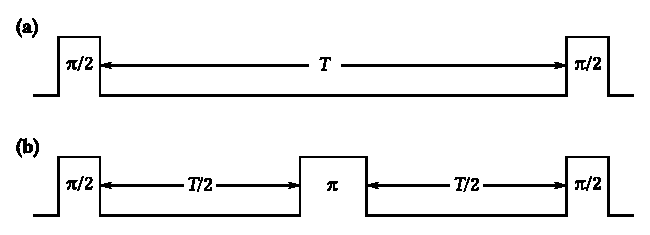
\includegraphics{figures_precreated/sequences.eps}}
    \caption{
    Timeline of the experiment for \textbf{(a)} the regular Ramsey sequence, and \textbf{(b)} the Ramsey sequence with spin echo.}
    \label{fig:bec-noise:visibility:sequences}
\end{figure}

The first protocol is the regular Ramsey sequence, depicted schematically in \figref{bec-noise:visibility:sequences},~(a): a $\pi/2$-pulse is applied by an electromagnetic coupler, creating a non-equilibrium superposition of components $\ket{1}$ and $\ket{2}$.
Mathematically, it means that coupling terms in~\eqnref{bec-noise:mean-field:cgpes-simplified} or in~\eqnref{bec-noise:wigner:single-particle-H} are enabled for a period of time equal to $t_{\mathrm{pulse}} = \theta / \Omega$, where $\theta = \pi/2$, and the Rabi frequency of the oscillator in this experiment was $\Omega = 350\un{Hz}$.
Since this pulse is short as compare to the total evolution time, it was simulated via the application of the rotation matrix~\eqnref{bec-noise:mean-field:rotation-matrix}.

During the further evolution of the system the components experience complex dynamics, separating and merging periodically~\cite{Mertes2007}.
This, in turn, leads to periodic dephasing and self-rephasing of the \abbrev{bec} components.
After some period of the free evolution the second $\pi/2$-pulse is applied, transforming the phase difference between the two components in the superposition into the population difference which can be imaged.
Many such experiments are performed with different free evolution times, contributing one time-point each, because the imaging effectively destroys the \abbrev{bec}.
A more detailed description of the experiment can be found in~\cite{Egorov2011} and in M.~Egorov's PhD thesis~\cite{Egorov2012}.

The simulations in this and the following sections used the plane wave basis (see \appref{bases} for details) and a $64\times8\times8$ spatial grid.
The integration was performed using a low-dissipation 4th-order Runge-Kutta algorithm (see \appref{numerical} for details).

The rephasing cycles can be represented by a common interferometric quantity --- the fringe contrast, or visibility:
\begin{eqn}
\label{eqn:bec-noise:visibility:visibility}
    \mathcal{V}
    = \frac{2 \left| \int \langle \Psiop_1^\dagger \Psiop_2 \rangle \upd \xvec \right|}%
        {\int \langle \Psiop_1^\dagger \Psiop_1 + \Psiop_2^\dagger \Psiop_2 \rangle \upd \xvec},
\end{eqn}
where the denominator is just the total number of atoms in the system.
This quantity can be shown to be the envelope curve of the population fringes produced by the second $\pi/2$-pulse in the experiment.
In the mean-field model the required correlations are calculated simply as
\begin{eqn}
    \tilde{n}
    & = \langle \Psiop_1^\dagger \Psiop_2 \rangle \approx \Psi_1^* \Psi_2, \\
    n_j
    & = \langle \Psiop_j^\dagger \Psiop_j \rangle \approx \Psi_j^* \Psi_j.
\end{eqn}
In the Wigner representation we have to make the correlations symmetrically-ordered first, and then~\eqnref{wigner-bec:fpe-bec:moments} gives us
\begin{eqn}
    \tilde{n}
    & = \langle \Psiop_1^\dagger \Psiop_2 \rangle
    = \langle \symprod{ \Psiop_1^\dagger \Psiop_2 } \rangle
    \approx \Psi_1^* \Psi_2, \\
    n_j
    & = \langle \Psiop_j^\dagger \Psiop_j \rangle
    = \langle \symprod{ \Psiop_j^\dagger \Psiop_j }
        - \frac{\delta_{\restbasis_j}(\xvec, \xvec)}{2} \rangle
    \approx \pathavg{ \Psi_j^* \Psi_j } - \frac{M}{2V},
\end{eqn}
where we used the fact that $\delta_{\restbasis_j}(\xvec, \xvec) \equiv M / V$ in the plane wave basis, where $M$ is the number of modes (for the grid we use $M = 64 \times 8 \times 8 = 4096$), and $V$ is the volume of the simulation area.

\begin{figure}
    \centerline{%
    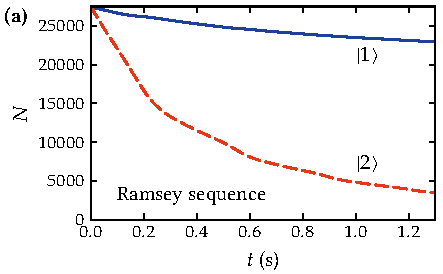
\includegraphics{figures_generated/bec_noise/ramsey_single_run_pop.pdf}%
    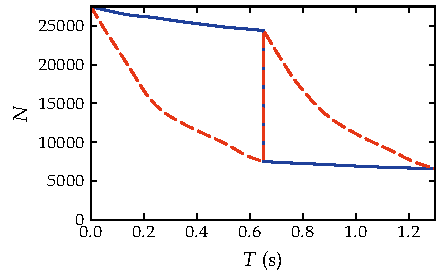
\includegraphics{figures_generated/bec_noise/echo_single_run_pop.pdf}}

    \caption{Numerically simulated population of components $\ket{1}$ (blue solid lines) and $\ket{2}$ (red dashed lines) in \textbf{(a)} Ramsey and \textbf{(b)} spin echo sequences.}

    \label{fig:bec-noise:visibility:population}
\end{figure}

\begin{figure}
    \centerline{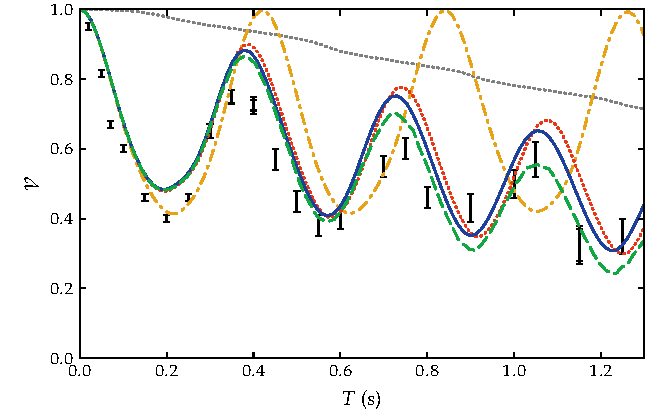
\includegraphics{figures_generated/bec_noise/ramsey_visibility_short.pdf}}

    \caption{
    Comparison of experimental and numerically simulated interferometric contrast at the end of a regular Ramsey sequence with the evolution time $t$.
    Experimental results (black bars) are shown in comparison with the results given by the mean-field model (green dotted line), truncated Wigner method (red dashed line), and truncated Wigner with technical noises included (blue solid line).
    The mean-field results with losses turned off (yellow dash-dotted line) and the population-dependent visibility limit~\eqnref{bec-noise:visibility:limit} (grey dotted line) are included as a reference.}

    \label{fig:bec-noise:visibility:ramsey-visibility}
\end{figure}

The visibility can serve as a good example of the differences introduced by taking into account losses, quantum effects, and technical noises in the simulation of the experiment.
The inclusion of these factors in the simulation of the Ramsey sequence is demonstrated in~\figref{bec-noise:visibility:ramsey-visibility}.
The experimental results and their uncertainties are shown as the black bars in the figure.

The simplest model --- the mean-field \abbrev{cgpe}s~\eqnref{bec-noise:mean-field:cgpes-simplified} with losses turned off --- gives results that are completely off base: the visibility is completely restored during rephasings (yellow dash-dotted lines in the figure).
This is to be expected, as the theoretical limit of visibility
\begin{eqn}
\label{eqn:bec-noise:visibility:limit}
    \mathcal{V}_{\mathrm{max}}
    = \frac{2 \sqrt{N_1 N_2}}{N_1 + N_2},
\end{eqn}
where $N_1$ and $N_2$ are populations before the second $\pi/2$-pulse, equals to $1$ in this case, and there are no other limiting factors.

But in the experiment in question the losses are present and are significantly asymmetrical, as shown in~\figref{bec-noise:visibility:population},~(a).
With the populations typical for the experiment (tens of thousands of atoms or less) the two-body loss process in $\ket{2}$ is significantly stronger than the three-body one in $\ket{1}$.
This makes the theoretical limit~\eqnref{bec-noise:visibility:limit} decrease with time, as the dotted grey line in~\figref{bec-noise:visibility:ramsey-visibility} shows.
The resulting mean-field prediction with the inclusion of nonlinear losses (green dotted lines) is much closer to the experimental data.

The application of the \abbrev{sde}s~\eqnref{bec-noise:wigner:sde} obtained with the Wigner method (red dashed lines) has little effect on the short-time visibility (although it becomes more important at longer times, as we will see later in~\figref{bec-noise:visibility:visibility-long}).
The Wigner results can be further adjusted to account for the noise introduced by the final measurement and non-ideal coupling (blue solid lines), which will be explained in detail in the next section.

The final agreement with the experiment is still not ideal, and the explanation of this difference is an open question.
Candidate factors include finite temperature effects and interaction with the surrounding cloud of non-condensed atoms.

\begin{figure}
    \centerline{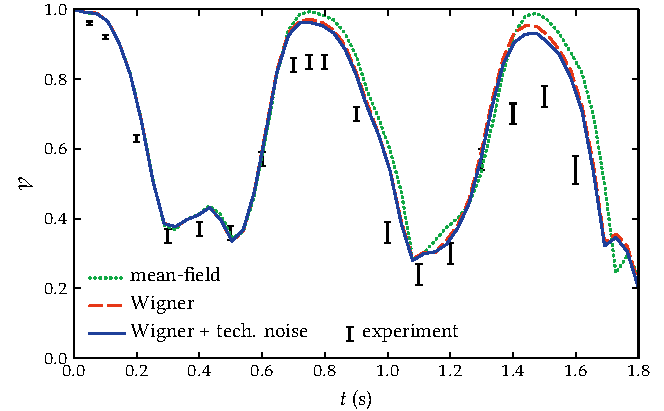
\includegraphics{figures_generated/bec_noise/echo_visibility_short.pdf}}

    \caption{Comparison of experimental and numerically simulated interferometric contrast at the end of a spin echo sequence with the evolution time $t$.
    Experimental results (black bars) show the final visibility value for a single spin echo sequence with the full evolution time $t$ as compared with the predictions from the mean-field model (green dotted line), truncated Wigner method (red dashed line), and truncated Wigner with technical noises included (blue solid line).}

    \label{fig:bec-noise:visibility:echo-visibility}
\end{figure}

The asymmetricity introduced by the difference in loss rates can be compensated by periodically swapping the populations of the two components by a ``spin echo'' coupler pulse of the length $\pi$.
The simplest, yet already very effective, variant is to apply the $\pi$-pulse in the middle of the evolution, as illustrated by~\figref{bec-noise:visibility:sequences},~(b).
With this additional pulse by the end of a single experimental sequence the populations of two components become equal again, as shown in~\figref{bec-noise:visibility:population},~(b), setting the theoretical visibility limit~\eqnref{bec-noise:visibility:limit} back to $1$.

The mean-field model predicts the full recovery of the visibility even at long evolution times, which is inconsistent with the experiment, as seen in~\figref{bec-noise:visibility:echo-visibility}.
On the other hand, the quasiprobability model qualitatively predicts the decay of visibility with time.
Same as in the case of the regular Ramsey sequence, the predictions of the simulation can be improved by including the technical noise.

\begin{figure}
    \centerline{%
    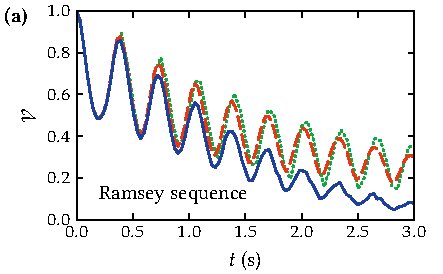
\includegraphics{figures_generated/bec_noise/ramsey_visibility_long.pdf}%
    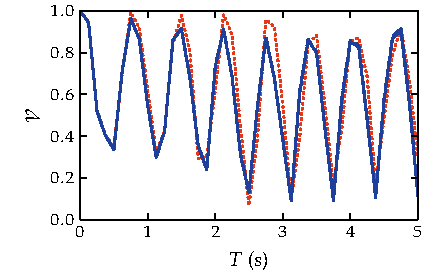
\includegraphics{figures_generated/bec_noise/echo_visibility_long.pdf}}

    \caption{Numerically simulated interferometric contrast for \textbf{(a)} a Ramsey sequence, and \textbf{(b)} a spin echo sequence at longer times.
    Mean-field (green dotted lines), truncated Wigner (red dashed lines) and truncated Wigner with technical noises (blue solid lines) are plotted.}

    \label{fig:bec-noise:visibility:visibility-long}
\end{figure}

The simulations can be performed for longer times, as shown in~\figref{bec-noise:visibility:visibility-long}.
The difference between the mean-field and the truncated Wigner approach becomes more clear in~\figref{bec-noise:visibility:visibility-long},~(a), where the truncated Wigner predicts the significant decrease in the amplitude of the rephasing oscillations, caused by the quantum noise.
One must remember though that at such times the simulated atom densities become too low due to losses and violate the truncation validity criterion~\eqnref{wigner-bec:truncation:delta-condition}, thus making the predictions less reliable.

% =============================================================================
\section{Phase noise}
% =============================================================================

Another important characteristic of a \abbrev{bec} interferometry experiment is the phase noise, which is connected with the visibility.
We will discuss it based on the same experiment~\cite{Egorov2011,Egorov2012} as in the previous section.

While in the simulation we can measure the visibility~\eqnref{bec-noise:visibility:visibility} simply by calculating a second-order moment, experimentalists do not have the luxury of knowing the wavefunctions of the components.
Instead, multiple runs of the Ramsey sequence with the same evolution time are performed, with the second $\pi/2$-pulse having a different phase lag $\phi$ each time.
The quantity that can be measured in the experiment is the normalized atom difference
\begin{eqn}
    P_z = \frac{N_2^\prime - N_1^\prime}{N_1^\prime + N_2^\prime},
\end{eqn}
where $N_1^\prime$ and $N_2^\prime$ are populations of the components obtained by imaging after the second $\pi/2$-pulse.
Using the rotation matrix~\eqnref{bec-noise:mean-field:rotation-matrix} it can be shown that $P_z$ can be expressed in terms of wave operators before the second $\pi/2$-pulse as
\begin{eqn}
    P_z(\phi)
    = - \frac{2}{N_1 + N_2} \Imag \left(
        e^{-i\phi} \int \langle \Psiop_1^\dagger \Psi_2 \rangle \upd\xvec
        \right).
\end{eqn}
One can notice that the integral of the second order moment in this expression is the same as in~\eqnref{bec-noise:visibility:visibility}, and is also normalized on the total population.
Therefore if we vary $\phi$ in the experiment, the resulting $P_z(\phi)$ can be fit with a sine function, and its amplitude will give us the visibility $\mathcal{V}$.

\begin{figure}
    \centerline{%
    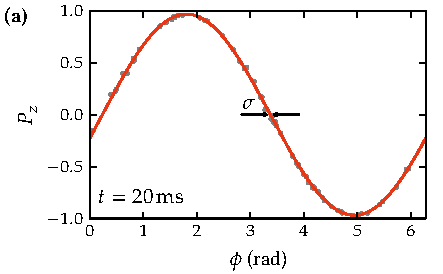
\includegraphics{figures_generated/bec_noise/illustration_noise_20ms.pdf}%
    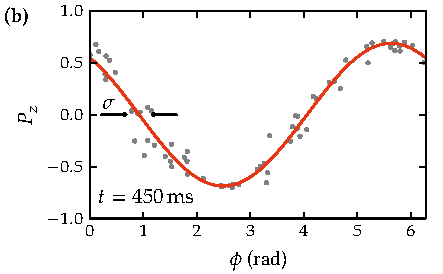
\includegraphics{figures_generated/bec_noise/illustration_noise_450ms.pdf}}

    \caption{Phase noise in experimental measurements of visibility at \textbf{(a)}~$t = 20\un{ms}$ and \textbf{(b)}~$t = 450\un{ms}$.
    Black dots illustrate possible results obtained in a single run of the Ramsey interferometry experiment.}%endcaption

    \label{fig:bec-noise:phase-noise:illustration}
\end{figure}

In practice, naturally, the measurement of $P_z$ is affected by various sources of technical noise.
As a result, the measured points are displaced from the ideal curve.
In the experiment in question three such noise sources were identified.
First, the length of $\pi/2$-pulses varied throughout the exeprimental runs with an estimated standard deviation of $\Delta \theta = 0.02\un{rad}$ (caused by the drift of the Rabi frequency $\Omega$).
The phase of the coupler also had an uncertainty caused by the MW frequency instability that grew with time as $\Delta \phi / t = 0.5\un{rad/s}$.
Finally, the imaging technique used to measure populations $N_1^\prime$ and $N_2^\prime$ resulted in an uncertainty of $\Delta N / N = 0.023$.
These factors can be trivially added to the simulations: first two at the moment of the application of the rotation matrix~\eqnref{bec-noise:mean-field:rotation-matrix}, by adding a random factor to the length $\theta$ and the phase $\phi$, and the third one by adding a random factor to the populations $N_1$ and $N_2$ produced by integrating the corresponding moments of wavefunctions.

The result is is illustrated in~\figref{bec-noise:phase-noise:illustration}, with the ``experimental'' points emulated this way plotted agains a sine fit, for two different evolution times.
The base simulation is the truncated Wigner one for the regular Ramsey sequence from the previous section.
The standard deviation of the horizontal distance $\sigma$ of the experimental results from the fitting curve is called the phase noise.
The amplitude of the curve, in turn, is taken to be the predicted visibility accounting for the technical noises (see~\figref{bec-noise:visibility:ramsey-visibility} and~\figref{bec-noise:visibility:echo-visibility} in the previous section).

\begin{figure}
    \centerline{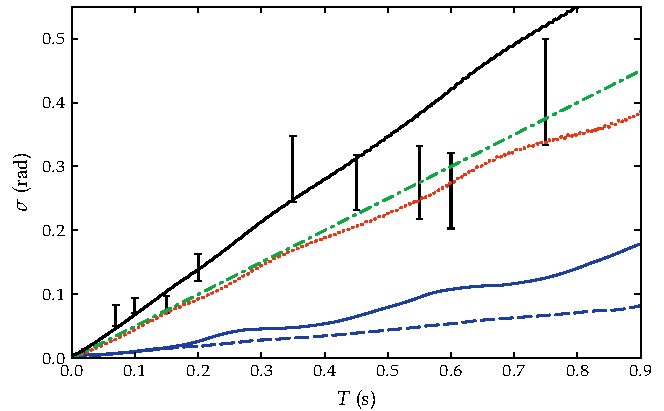
\includegraphics{figures_generated/bec_noise/ramsey_noise.pdf}}

    \caption{Comparison of experimental (black bars) and numerically simulated phase noise at the end of a Ramsey sequence with the evolution time $t$.
    The truncated Wigner predictions with (blue solid line) and without (red dashed line) the inclusion of technical noises is shown.}%endcaption

    \label{fig:bec-noise:phase-noise:ramsey-phnoise}
\end{figure}

A comparison of the phase noise with the experimental data for the regular Ramsey sequence is shown in~\figref{bec-noise:phase-noise:ramsey-phnoise}.
The experimental parameters are the same as in the previous section.
The effect of quantum noise (red dashed line) is noticeable, but not very large as compared to the compound effect of the technical noises (blue solid line).
There seems to be a lot of room for the improvement of the apparatus until the measurements hit the ``hard'' limit of the quantum noise.

\begin{figure}
    \centerline{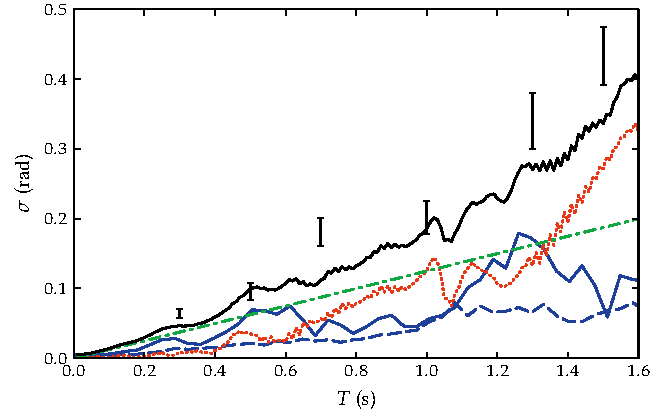
\includegraphics{figures_generated/bec_noise/echo_noise.pdf}}

    \caption{Comparison of experimental (black bars) and numerically simulated phase noise at the end of a spin echo sequence with the evolution time $t$.
    The truncated Wigner predictions with (blue solid line) and without (red dashed line) the inclusion of technical noises is shown.}%endcaption

    \label{fig:bec-noise:phase-noise:echo-phnoise}
\end{figure}

Phase noise in a spin echo sequence can be estimated in the same way.
The reported MW frequency instability for this experiment was $\Delta \phi / t = 0.125\un{rad/s}$.
As~\figref{bec-noise:phase-noise:echo-phnoise} shows, even after the inclusion of the technical noise, there is some disagreement with the experimental data.
This may be caused by the systematic error introduced by the truncation, or possibly by some additional source of technical noise.

One may notice that the total noise shown in~\figref{bec-noise:phase-noise:ramsey-phnoise} and~\figref{bec-noise:phase-noise:echo-phnoise} is lower than the one reported in~\cite{Egorov2011,Egorov2012}.
This is the result of the honest calculation of the total noise (in essence, we simulate the actual experimental measurement procedure), as opposed to the post-factum combination of noise from the technical sources with the Wigner results.

% =============================================================================
\section{Conclusion}
% =============================================================================

The examples in this chapter demonsrate that the truncated Wigner approach gives correct long-time predictions of quantum effects for the system comprised of large number of atoms.
Both of these features, large atom numbers and long time-scales, are essential to accurate interferometric measurements.
The predictions remains correct even despite multimode dynamical motion in three dimensions and substantial losses of most of the condensate atoms.
On longer time-scales, the experimental accuracy is limited by technical noises, and we have no data for comparisons.

